\section{Benefit analysis}
\label{sec:benefit_analysis}

\subsection{Comparable benchmarks}
The following studies are a subset of benchmarks that show the potential of precision medicine, particularly through genomic sequencing and multi-omic technologies, in diagnosing and managing rare and complex conditions. 
By implementing known methods, we can improve patient outcomes, enable targeted therapies, and potentially reduce healthcare costs through more accurate and faster diagnoses.
This integration promises not only to improve patient care but also to provide critical insights into the genetic basis of diseases, ultimately informing both treatment and prevention strategies.

\subsection*{Economic impact of sepsis - \citep{van2022hospital}}
\begin{itemize}
  \item \textbf{Patient data and impact}: Review covers studies reporting costs associated with adult sepsis patients globally, indicating significant economic burden.
  \item \textbf{Methodology}: Systematic review under PRISMA guidelines, with data from PubMed, EMBASE, and Cochrane.
  \item \textbf{Key statistics}: Reports wide cost range from €1,101 to €91,951 per sepsis patient, reflecting international healthcare system variances.
\end{itemize}

\subsection*{Genomic insights in critical care for infants - \citep{meng2017use}}
\begin{itemize}
  \item \textbf{Patient data and impact}: Involves 278 critically ill infants; molecular diagnosis achieved in 36.7\% of cases, with higher rates (50.8\%) in critical trio exome cases.
  \item \textbf{Methodology}: Utilises proband exome, trio exome, and critical trio exome sequencing.
  \item \textbf{Key statistics}: Impacted medical management in 52.0\% of diagnosed cases.
\end{itemize}

\subsection*{National scale multi-omics for rare diseases - \citep{lunke2023integrated}}
\begin{itemize}
  \item \textbf{Patient data and impact}: Involves 290 critically ill infants and children; diagnostic yield from WGS initially at 47\%, increased to 54\% with extended analysis.
  \item \textbf{Methodology}: Rapid whole-genome sequencing integrated with transcriptomic data.
  \item \textbf{Key statistics}: Altered critical care management in 77\% of diagnosed cases.
\end{itemize}

\subsection*{Genomic lifespan association in Iceland - \citep{jensson2023actionable}}
\begin{itemize}
  \item \textbf{Patient data and impact}: Study includes 57,933 participants, identifying 2,306 individuals with actionable genotypes.
  \item \textbf{Methodology}: Whole-genome sequencing focusing on 73 genes from ACMG Secondary Findings recommendations.
  \item \textbf{Key statistics}: Actionable genotypes linked to a decrease in median lifespan by approximately three years for carriers.
\end{itemize}

\subsection*{Genome analysis in neurodevelopmental disorders - \citep{sanchis2023genome}}
\begin{itemize}
  \item \textbf{Patient data and impact}: Encompasses 465 families, finding causal variants in 36\% of 489 affected individuals.
  \item \textbf{Methodology}: Combines short-read and long-read genome sequencing.
  \item \textbf{Key statistics}: Long-read sequencing crucial for resolving complex variants.
\end{itemize}

\subsection*{Rapid whole-genome sequencing in UAE - \citep{abou2023rapid}}
\begin{itemize}
  \item \textbf{Patient data and impact}: Initial feasibility study with five infants, three of whom were successfully diagnosed.
  \item \textbf{Methodology}: Rapid whole-genome sequencing with a turnaround of 37 hours on average.
  \item \textbf{Key statistics}: Demonstrates the utility of rWGS in diverse populations within a Middle-Eastern context.
\end{itemize}

\subsection*{Genome sequencing for rare diseases - \citep{wojcik2024genome}}
\begin{itemize}
  \item \textbf{Patient data and impact}: Involves 822 families with rare monogenic diseases, achieving a diagnostic yield of 29.3\%.
  \item \textbf{Methodology}: Focuses on broader genomic coverage including structural and non-coding variants.
  \item \textbf{Key statistics}: Identifies causative variants in 8.2\% of cases previously undetected by exome sequencing.
\end{itemize}

\subsection*{UK and Ireland genomic diagnostics in paediatrics - \citep{wright2023genomic}}
\begin{itemize}
  \item \textbf{Patient data and impact}: The DDD study involved over 13,500 families; approximately 41\% of probands received a genetic diagnosis.
  \item \textbf{Methodology}: Integrated genomic data analysis with clinical phenotyping.
  \item \textbf{Key statistics}: Highlights cost-saving potential through precise diagnostics and targeted therapy.
\end{itemize}

\subsection{Introduction to source data by Federal Statistical Office}
The following data are based on statistics reported by Bundesamt für Gesundheit (BAG), \url{https://www.bag.admin.ch/} for years 2010-2022. 
We gathered the yearly statistics for all hospitals and clinics which are gathered for
Statistiken zur Krankenversicherung, Qualitätsindikatoren der Schweizer Akutspitäler.

The Bundesamt für Gesundheit (BAG) or Federal Office of Public Health (FOPH), under the mandate of the Federal Department of Home Affairs (FDHA), published quality indicators for hospitals for the first time in 2009 as part of a pilot project. This initiative is based on the revised Federal Health Insurance Act (LAMal), which mandates the publication of data on the quality and cost-effectiveness of service providers.

In collaboration with the Federal Statistical Office (FSO), FOPH chose to adopt the quality indicator concept used by the German HELIOS Clinics. This concept is based on various internationally recognized systems, such as the AHRQ IQIs (Agency for Healthcare Research and Quality - Inpatient Quality Indicators) from the United States and is also utilized by the Quality Medicine Initiative (IQM) in Germany and nationally in Austria. This approach provides Swiss hospitals with a basis for international comparison, particularly benefiting the five Swiss university hospitals by allowing a comparison of their outcomes with those published online from leading German clinics. The indicators are analyzed using existing routine data collected in cooperation with the cantons by the FSO in the Medical Statistics of Hospitals.

With this approach, FOPH enables a systematic, nationwide comparison of outcome quality in acute care hospitals. The Swiss hospital data, which encompasses comprehensive case data in the inpatient sector, is crucial for enabling a thorough comparison based on these routine data. The IQI systems are jointly revised and expanded in Germany and Switzerland. For the current evaluation, the CH-IQI specifications version 5.4 served as the basis for calculations. The indicators provide valuable insights into individual hospital performances and potential areas for improvement, although they do not allow a conclusive judgment on the quality of care provided by hospitals.








\subsection{Analysis results for \pmu}
Time series was performed using linear regression (for cost analysis) and Poisson regressions (for mortality  to extrapolate the expected outcomes from 2010-2030.
The actual cost and number of cases in for the past 12 years is accurately reported by BAG, however or estimate for future savings and benefit depend on the achievable benchmarks reported in the  sections of \ref{sec:benefit_analysis}.
As our number update, we can build a more reliable model of what to expect over the next 10 years. 
The \pmu cost analysis overview is shown in figure 
\ref{fig:cost_analysis}.

\begin{figure}[h] \hspace*{0cm} 
\begin{center}
	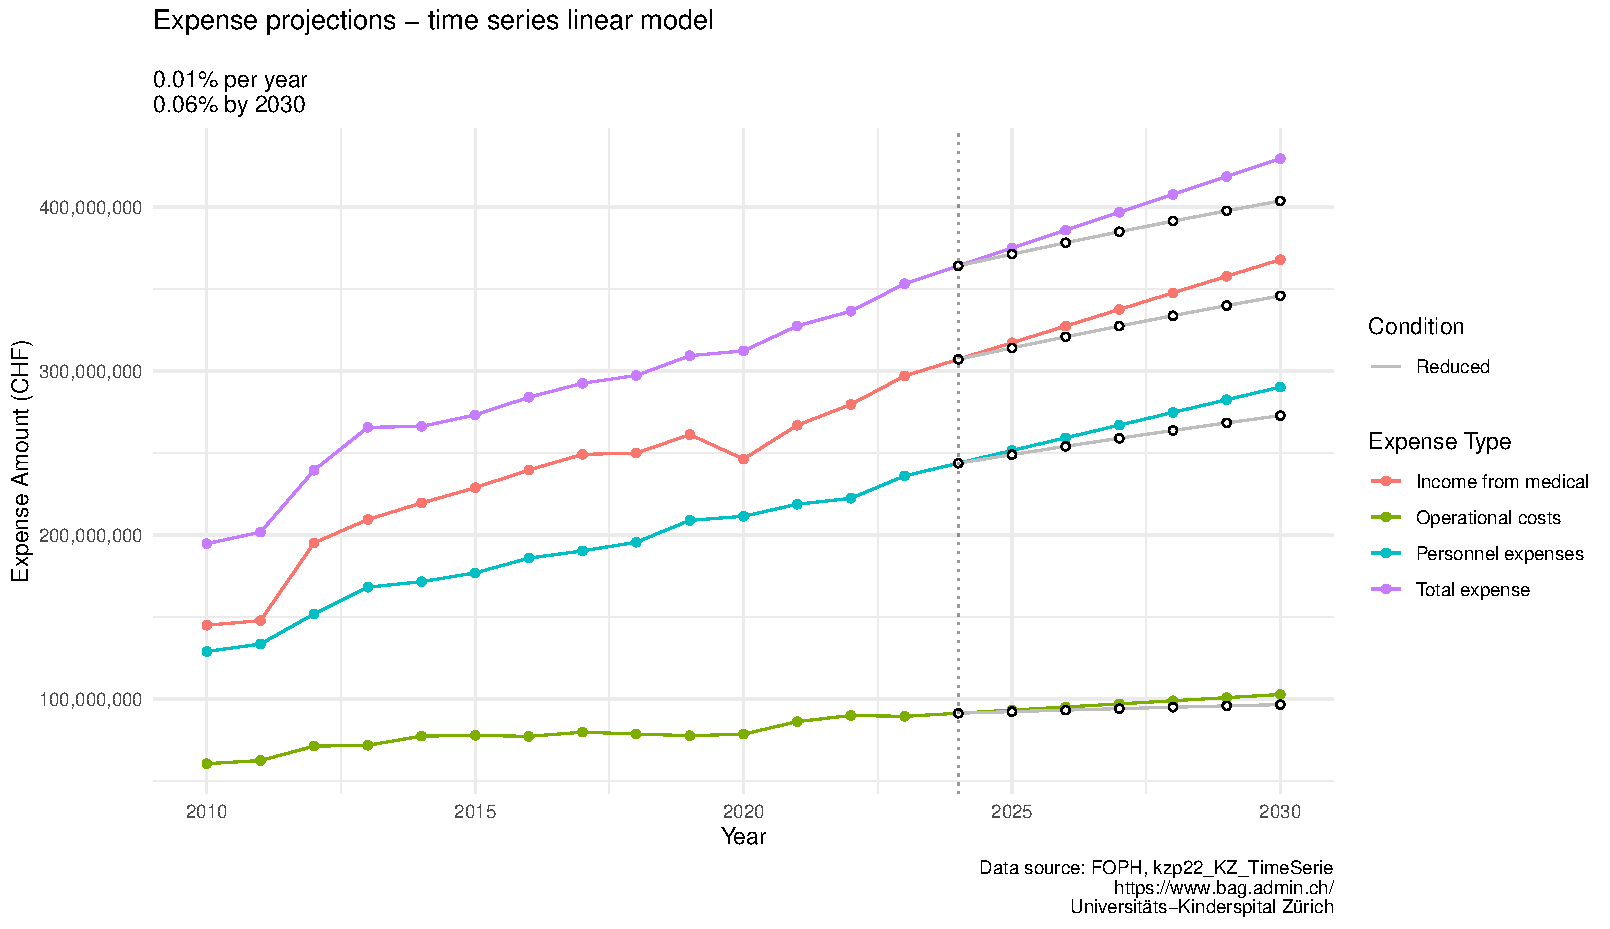
\includegraphics[width=0.90\textwidth]{../stats/foph_key_stats/output/p_cost}
	\caption{Projections for Kispi with a \pmu (2010-2030). Federal statistics from Bundesamt für Gesundheit (BAG, Federal office for public health) were modelled and projected to 2030. A modest benefit effect size was applied. 
	In the most similar application to our \pmu; 
	\citet{lunke2023integrated} 
	showed a 54\% diagnostic yield and an altered critical care management in 77\% of diagnosed cases.
	We estimated modest 1\% increase in actualised savings per year after successful implementation starting in 2024.}
	\label{fig:cost_analysis}
\end{center}
\end{figure}

A more accurate demonstration of the \pmu can be seen with a specific disease example using sepsis.
Sepsis was specifically modelled using federal statistics from Bundesamt für Gesundheit (BAG, Federal office for public health) from 2010-2022 as shown in 
\textbf{figures
\ref{fig:p_cases_sepsis_uni_yearly},
\ref{fig:p_cases_sepsis_kispi_yearly_forecast},
\ref{fig:p_cases_per_indicator_kispi_2022}}.

First we get a global picture of sepsis in University hospitals in 
\textbf{figure
\ref{fig:p_cases_sepsis_uni_yearly}}. 
This illustrates the total number of sepsis in adult and paediatric settings across the country.
\textbf{Figure \ref{fig:p_cases_sepsis_kispi_yearly_forecast}} 
shows a forecast model, from 2010-2030, for the number of deaths due to sepsis in \kispi
(repeated from executive summary).
The predicted number of prevetable deaths is based on comparable benchmarks listed in section 
\textbf{\ref{sec:benefit_analysis}} 
which have demonstrated clear cost-saving potential through precise diagnostics and targeted therapy.
For rare diseases, approximately 40\% of probands received a genetic diagnosis 
\citep{wright2023genomic, wojcik2024genome}
and altered critical care management in 77\% of diagnosed cases \citep{lunke2023integrated}.
A well-managed work-flow can result in rapid whole-genome sequencing with a turnaround of 37 hours on average
 \citep{abou2023rapid}.
Based on such values, the forecast  projected into 2030 shows the yearly cases of sepsis.
Black and red values show the expected number of deaths with and without  precise diagnostics and targeted therapy, respectively. 

\begin{figure}[h] \hspace*{0cm} 
\begin{center}
	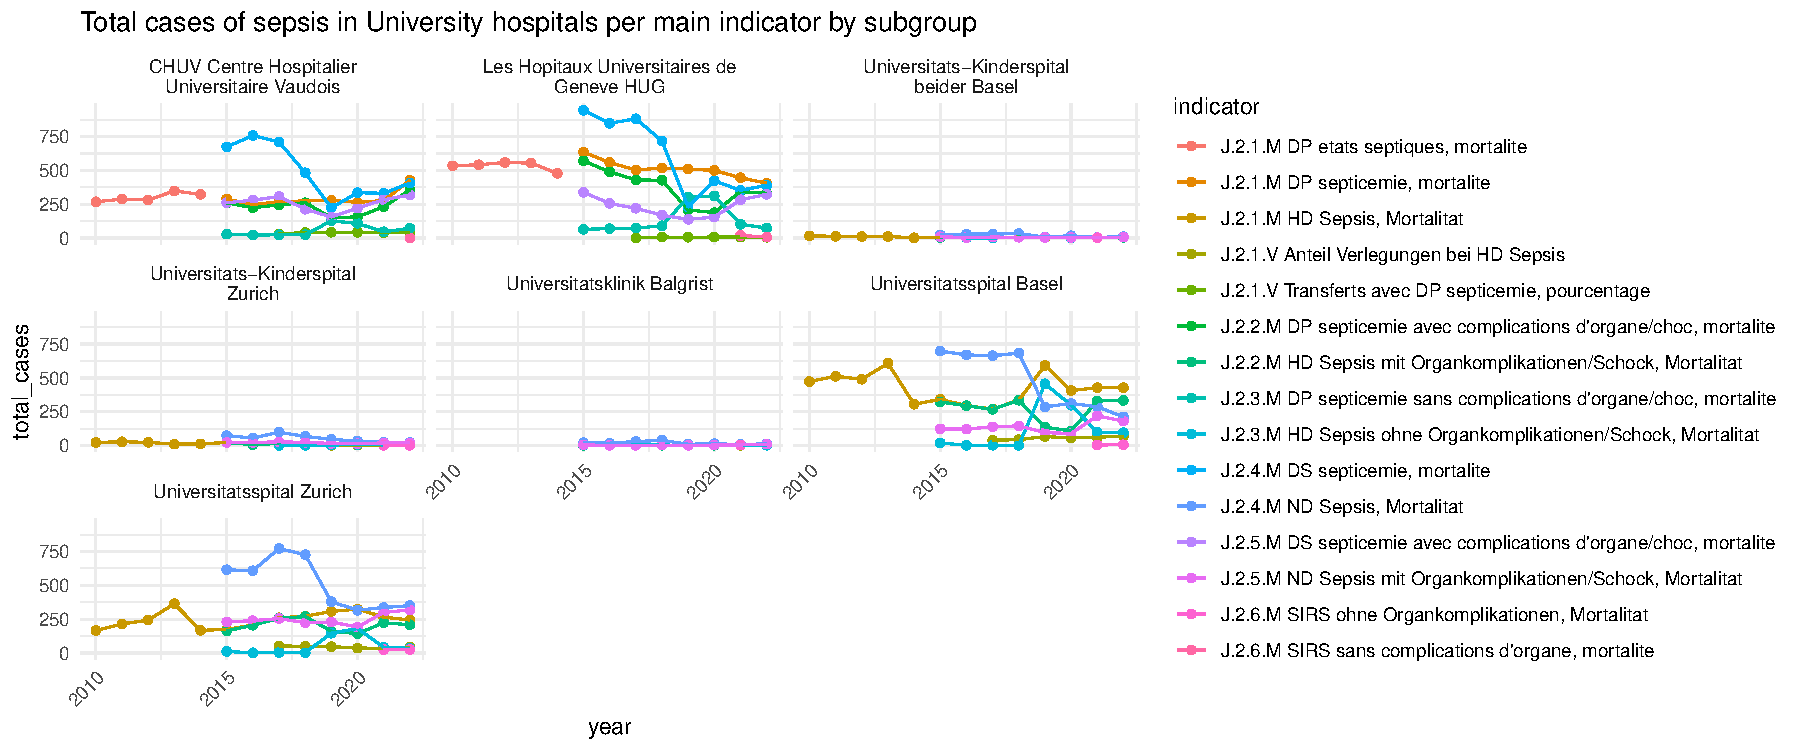
\includegraphics[width=1\textwidth]{../stats/foph_key_stats/output/p_cases_sepsis_uni_yearly}
	\caption{Yearly deaths due to sepsis at University hospitals across Switzerland.
	This data is based on statistics reported by Bundesamt für Gesundheit (BAG), 
	\url{https://www.bag.admin.ch/} for years 2010-2022. 
		DP: Diagnostic procedure.
HD: Primary diagnosis.
ND: Secondary diagnosis.}
	\label{fig:p_cases_sepsis_uni_yearly}
\end{center}
\end{figure}

\begin{figure}[h] \hspace*{0cm} 
\begin{center}
	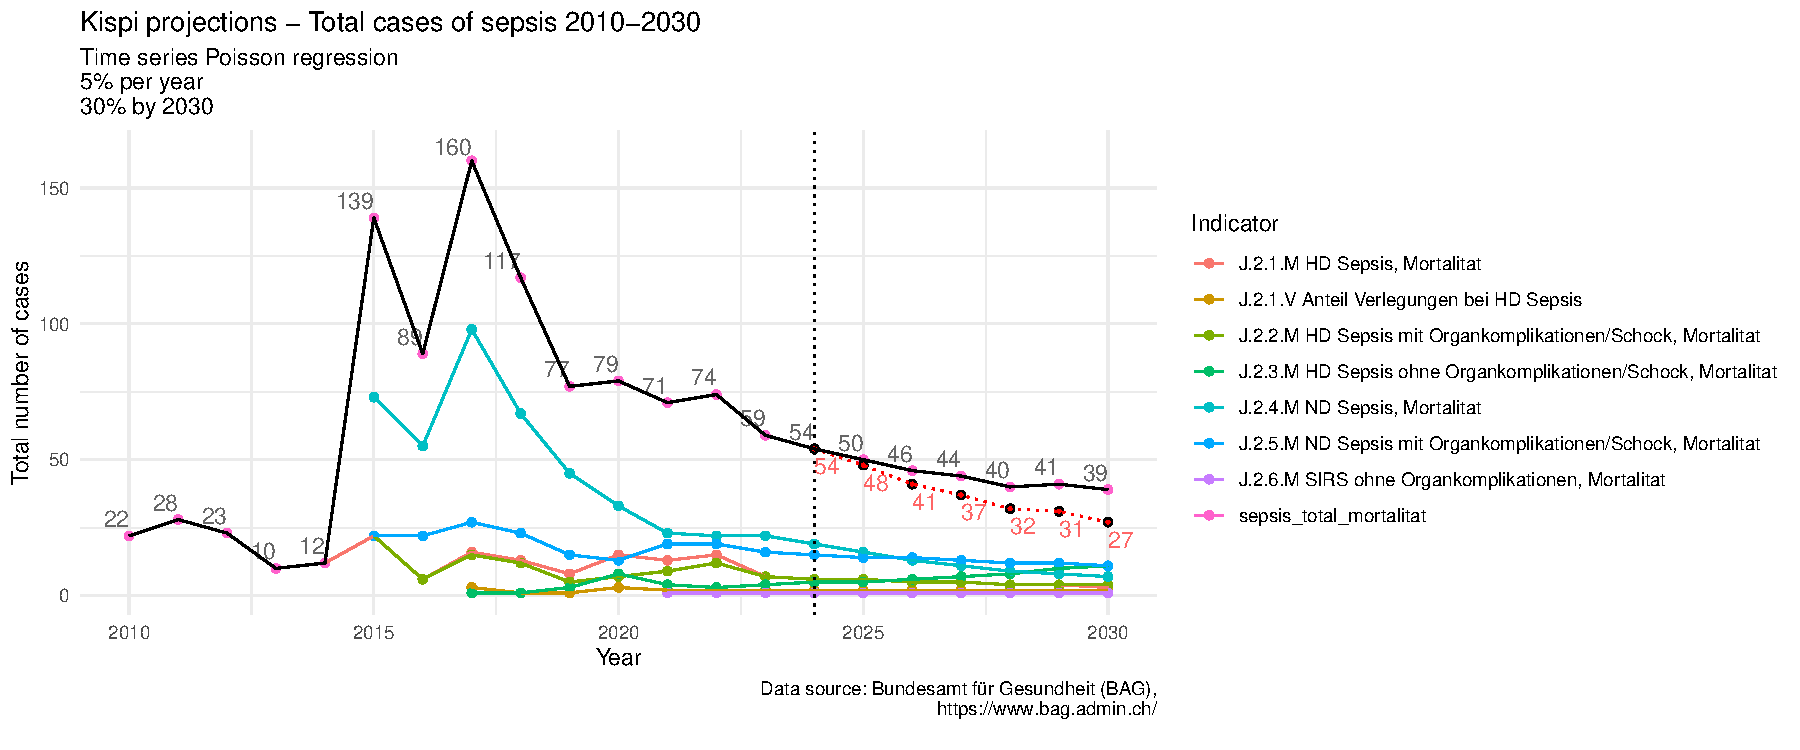
\includegraphics[width=1\textwidth]{../stats/foph_key_stats/output/p_cases_sepsis_kispi_yearly_forecast}
	\caption{Yearly deaths due to sepsis at \kispi.
	This data is based on statistics reported by Bundesamt für Gesundheit (BAG), 
	\url{https://www.bag.admin.ch/} for years 2010-2022. 
	Time series was performed using Poisson regression to extrapulate the expected outcomes from 2010-2030.
	Predictions for the cost and number of cases were generated in section 
	\ref{sec:benefit_analysis}.	
	DP: Diagnostic procedure.
HD: Primary diagnosis.
ND: Secondary diagnosis.}
	\label{fig:p_cases_sepsis_kispi_yearly_forecast}
\end{center}
\end{figure}

To put the work of the \pmu in perspective, we look at the total number case statistics for \kispi.
We see a total number of all cases indicators in 2022 of \textbf{10'261}.
The subgroup indicator for ``J.2 sepsis'' shows \textbf{74} cases in 2022.
\textbf{Figure \ref{fig:p_cases_per_indicator_kispi_2022}}  shows the the indicators through A1-Z4, many of which are similarly affected by the advances in precision medicine and are thus potential future prospects.

\begin{itemize}
\item \textbf{J} - ``Affections complexes, hétérogènes (indicateur pour peer review)'' or ``Complex, heterogeneous conditions''.
\begin{itemize}
	\item  \textbf{J.1} - ``Beatmung und extrakorporale Verfahren'', or ``Artificial respiration and extracorporeal procedures''.
	\item  \textbf{J.2} - ``Sepsis''.
	\item  \textbf{J.3} - ``Constellations complexes'', or ``Multifactorial Conditions''.
\end{itemize}
\end{itemize}

\begin{figure}[h] \hspace*{0cm} 
\begin{center}
	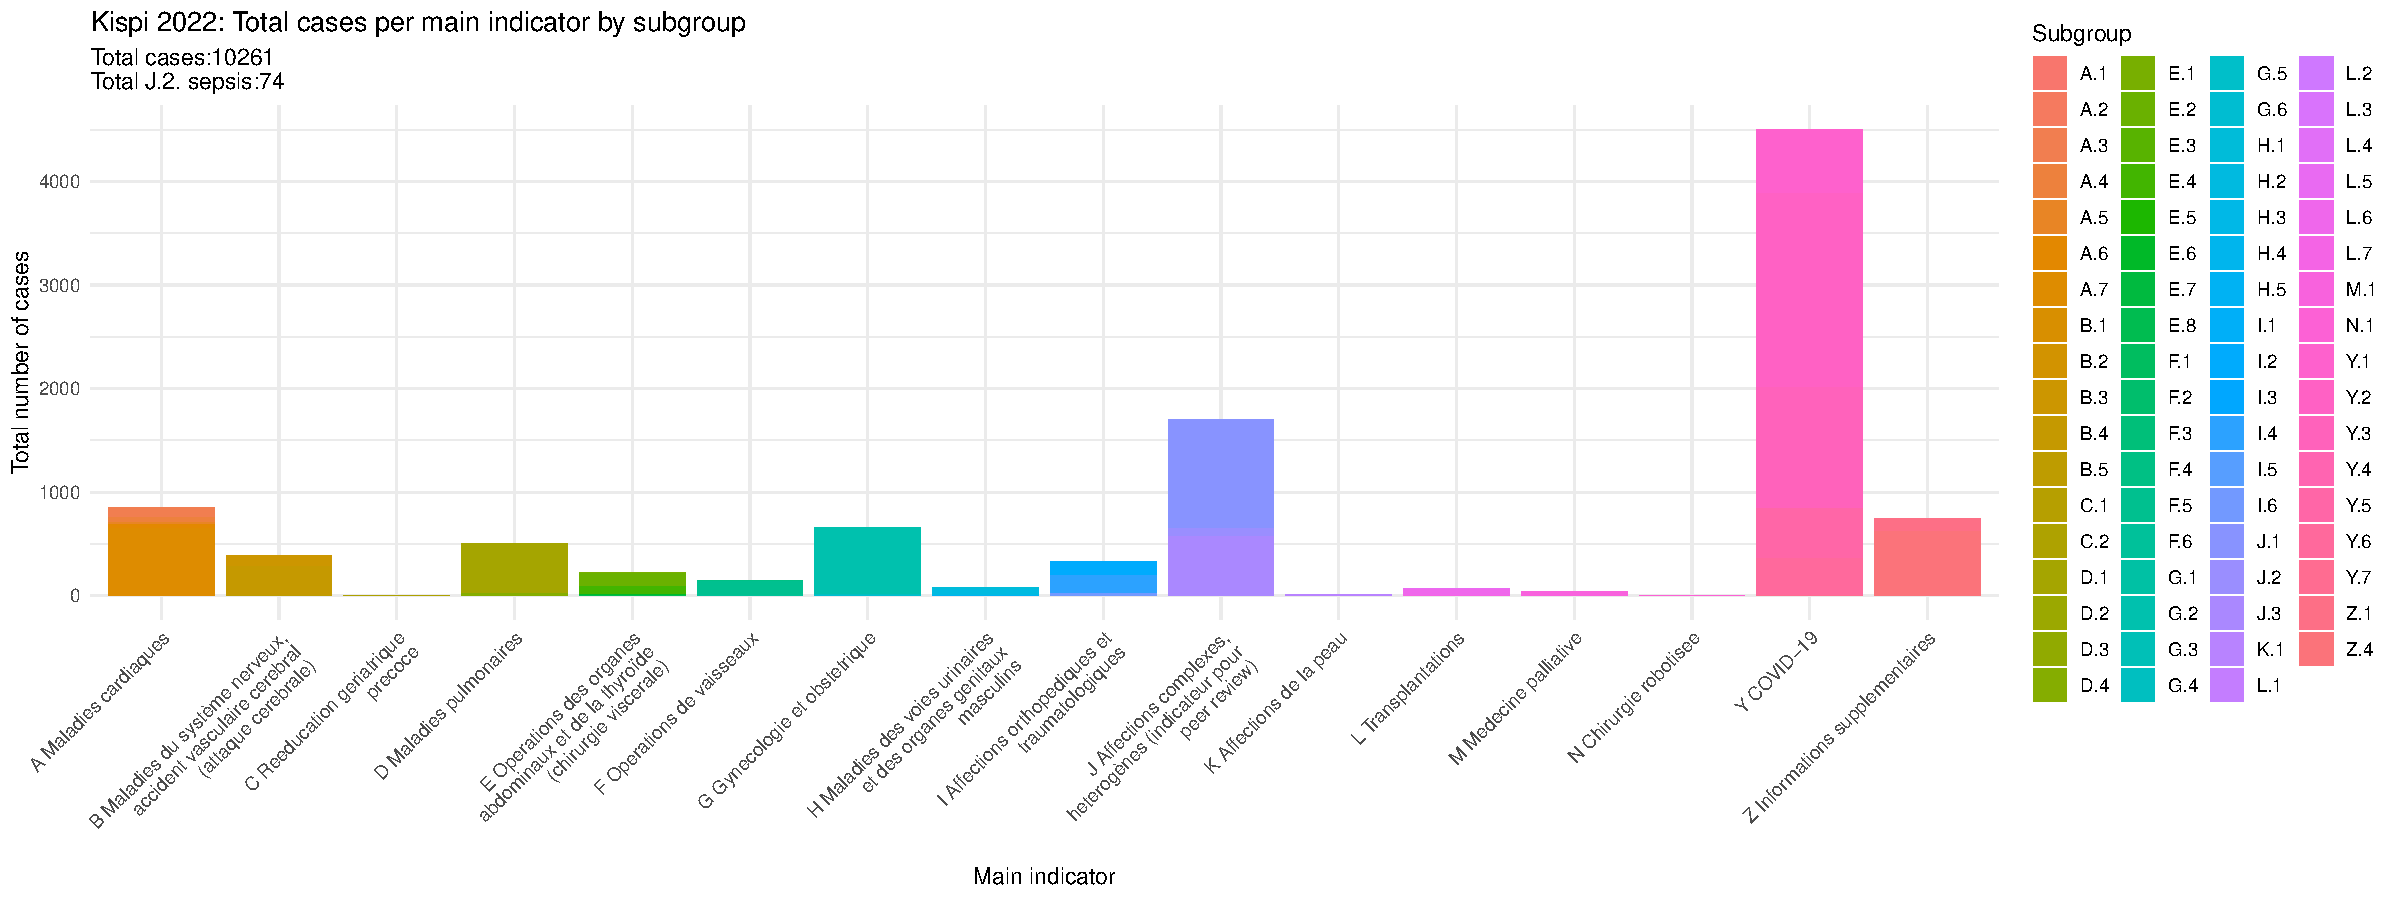
\includegraphics[width=1\textwidth]{../stats/foph_key_stats/output/p_cases_per_indicator_kispi_2022}
	\caption{The total count of case descriptions in \kispi for 2022 as categorised according to indicators for the Federal Statistical Office. 
	The `J.2 Sepsis` subset was used in the other figures shown in this section.}
	\label{fig:p_cases_per_indicator_kispi_2022}
\end{center}
\end{figure}

\clearpage